\documentclass[11pt,a4paper]{article}
\usepackage[T1]{fontenc}
\usepackage[utf8]{inputenc}
\usepackage{lmodern}
\usepackage{amsmath,amssymb,amsthm,mathtools,mathrsfs}
\usepackage{graphicx,float,xcolor,multicol}
\usepackage[shortlabels]{enumitem}
\usepackage[margin=27mm]{geometry}
\usepackage{microtype,needspace,placeins}
\usepackage{tikz,tikz-cd}
\usetikzlibrary{arrows.meta,calc,positioning,patterns,decorations.pathreplacing}
\usepackage[colorlinks=true,linkcolor=teal,urlcolor=teal,citecolor=teal]{hyperref}
\setlength{\parindent}{0pt}
\setlength{\parskip}{.6em}
\setcounter{secnumdepth}{0}
\allowdisplaybreaks
\raggedbottom
\providecommand{\cross}{\times}
\DeclareUnicodeCharacter{2020}{\ensuremath{\dagger}}
\DeclareMathOperator{\supp}{supp}
\DeclareMathOperator*{\esssup}{ess\,sup}
\providecommand{\chapter}{\section}
\newenvironment{tool}[2]{\subsection*{Tool #1 --- #2}}{}
\newcommand{\ToolRef}[1]{Tool #1}
\newcommand{\FigureTag}[2]{\textit{Figure #1}}
\newcommand{\Result}[1]{\subsection*{#1}}
\newcommand{\Application}[1]{\subsubsection*{Application\if\relax\detokenize{#1}\relax\else\space--- #1\fi}}
\newcommand{\ProofHeading}{\par\textit{Proof.}\space}
\newcommand{\ProofOf}[1]{\par\textit{Proof of #1.}\space}
\newcommand{\RemarkHeading}{\par\textbf{Remark.}\space}
\newcommand{\NoteHeading}{\par\textbf{Note.}\space}
\newcommand{\ExerciseHeading}{\par\textbf{Exercise.}\space}

\graphicspath{{figures/complex-analysis/}}
\begin{document}
\section*{Connectedness and Compactness}
% BLOG-CONTENT-BEGIN
\subsection*{Tool 2 — Real-Part Formula for the Modulus}
\[
|z|=\sup_{\theta}\operatorname{Re}\bigl(e^{i\theta}z\bigr).
\]


\begin{figure}[htbp]
  \centering
  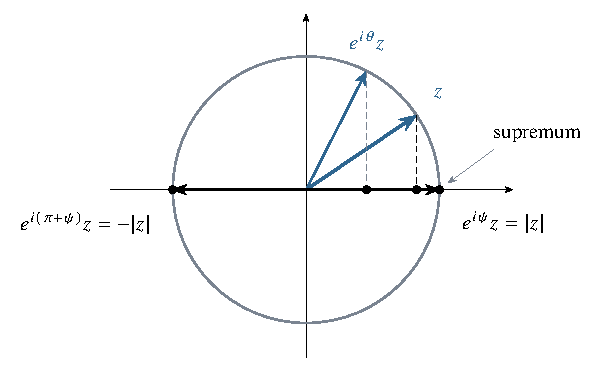
\includegraphics[width=0.72\linewidth]{note1-fig-01.pdf}

\end{figure}

Given a function $f\in L^1(\mu)$, we have,
\[
\left|\int_X f\,d\mu\right|\leq\int_X|f|\,d\mu.
\]

\textit{Proof.}
For every $\theta$,
\begin{align*}
\left|\operatorname{Re}\left(e^{i\theta}\int_Xf\,d\mu\right)\right|
&=\left|\int_X\operatorname{Re}(e^{i\theta}f)\,d\mu\right|\\
&\leq\int_X\left|\operatorname{Re}(e^{i\theta}f)\right|\,d\mu\\
&\leq\int_X|e^{i\theta}f|\,d\mu
=\int_X|f|\,d\mu.
\end{align*}
The first inequality is a consequence of the definition via simple functions. Taking the supremum in $\theta$ and applying Tool 2 proves the claim.

Thus, a result one might have for real-valued functions can pass through to complex-valued functions if Tool 2 can be applied.

\subsection*{Tool 3 — Continuous Images Preserve Connectedness}
The continuous image of a connected set is connected.


\subsection*{Tool 4 — Heine--Borel Theorem}
In $\mathbb R^n$, ``compact'' is equivalent to ``closed and bounded.''


These are basic topological facts.

\subsubsection*{Application — Connectedness and compactness}
Before seeing an application of Tool 3 and Tool 4, notice that Tool 2 exploits the rigidity of $\mathbb C$. Since the only origin-fixing isometries of $\mathbb C$ are reflections and rotations, we see that \(\{z:|z|=k\}\)
is, in fact, a circle.


There is no continuous function $f\colon\mathbb C^*\to\mathbb C^*$ such that \(f(z)^2=z\ \ (\forall z\in\mathbb C^*).\)
\textit{Proof.}
Assume the contrary. Then $-f$ is continuous. Define
\[
h\colon\mathbb C^*\times\{\pm1\}\longrightarrow\mathbb C^*,
\qquad
h(z,\sigma)=
\begin{cases}
f(z),&\sigma=1,\\
-f(z),&\sigma=-1.
\end{cases}
\]
The space $\mathbb C^*\times\{\pm1\}$ is, in a way, $\mathbb C^*\sqcup\mathbb C^*$. By the gluing lemma, $h$ is continuous. Also,
\begin{align*}
h(z,\pm1)=h(w,\pm1)
&\Longrightarrow h(z,\pm1)^2=h(w,\pm1)^2\\
&\Longrightarrow f(z)^2=f(w)^2
\Longrightarrow z=w,
\end{align*}
while
\[
h(z,1)=h(z,-1)
\Longrightarrow f(z)=-f(z)
\Longrightarrow f(z)=0,
\]
which is impossible. Hence $h$ is injective. Surjectivity is easily seen.

Consequently,
\[
h\big|_{S^1\times\{\pm1\}}
\]
is a homeomorphism between $S^1\times\{\pm1\}$ and $S^1$. By Tool 3, however, $S^1\times\{\pm1\}$ is not connected while $S^1$ is connected, a contradiction.

Thus ``$\log$'' cannot be defined on any domain containing $S^1$. In fact, there is the following general version.

\subsection*{General version}
There is a continuous branch of the logarithm, \(f\colon\Omega\longrightarrow\mathbb C,\)
for a domain $\Omega\subset\mathbb C\setminus\{0\}$ if and only if $\{0\}$ and $\{\infty\}$ belong to the same component of $\Omega^c$ in the Riemann sphere.

\textbf{Exercise.}
Use the general version to deduce the preceding nonexistence result.


Suppose \(f^2,\ \overline f\in H(\Omega).\)
Then $f\in H(\Omega)$; in fact, $f$ is constant.

\textit{Proof.}
Assume the fact that
\[
g,\overline g\in H(\Omega)\Longrightarrow g\text{ is constant}.
\]
Then
\[
f^2,(\overline f)^2\in H(\Omega)
\Longrightarrow
f^2,\overline{f^2}\in H(\Omega),
\]
so \(f^2(z)=c=re^{i\theta}\)
for some fixed $c$. Since $\overline f\in H(\Omega)$, writing
\[
\overline f=u-iv
\]
shows that $\overline f$ is continuous, hence $u$ and $v$ are continuous, and therefore $f=u+iv$ is continuous. Note that
\[
\frac{f}{\sqrt r\,e^{i\theta/2}}\in\{\pm1\}.
\]
Applying Tool 3 again gives
\[
f(z)=\sqrt r\,e^{i\theta/2}
\qquad\text{or}\qquad
f(z)=-\sqrt r\,e^{i\theta/2}.
\]

``Holomorphic and conjugate-holomorphic functions never vary together. Keep that as a rule of thumb.''

Prove that the only compact subgroups of $\mathbb C^*$ are $S^1$ and the groups of $n$th roots of unity.

\textit{Proof.}
Let $G$ be a compact subgroup of $\mathbb C^*$. If $z\in G$ with $|z|>1$, then \(\{z^n\}_n\subseteq G,\)
so $G$ is not bounded and, by Tool 4, is not compact. Similarly, if $z\in G$ and $|z|<1$, then $|1/z|>1$ and the same argument applies. Hence $G$ is a subgroup of $S^1$.

Let us argue that if $G\neq S^1$, then $G$ is finite. Suppose not. Since $G$ is infinite and compact, it has a limit point. Without loss of generality, assume $g_0=1$: if $g_n\to g_0$, then $g_ng_0^{-1}\to1$. Let $\varepsilon_k>0$ and consider $B_{\varepsilon_k}(1)\cap S^1$. Choose
\[
g=e^{i\theta}\in B_{\varepsilon_k}(1)\cap S^1.
\]


Choose $v\in S^1\setminus G$. There is a $k'$ with
\[
0\leq k'\leq\left[\frac{2\pi}{\theta}\right]
\]
such that, if $v=e^{i\psi}$, then
\[
k'\theta<\psi<(k'+1)\theta.
\]
Note that \(\left|e^{i(k'+1)\theta}-e^{ik'\theta}\right|<\varepsilon_k,\)
and hence
\[
\left|e^{i\psi}-e^{ik'\theta}\right|<\varepsilon_k,
\qquad
|v-g^{k'}|<\varepsilon_k.
\]
Set $\varepsilon_k=1/k$ to obtain a sequence $\{g_k\}_k$ with $g_k\to v$. Thus $v\in G$, a contradiction.

Note that \(\left\langle e^{i\theta}:\theta\in\mathbb Q\right\rangle\)
is a subgroup of $S^1$, essentially the union of all roots of unity, but it is not compact.

\textbf{Remark.}
Heine--Borel fails even for an infinite discrete space: the whole space is both closed and bounded, but it is not compact.

The only connected closed subgroups of $\mathbb C^*$ are
\[
\mathbb C^*,\qquad \langle1\rangle,
\qquad\text{and}\qquad
\left\langle \exp(tz):t\in\mathbb R\right\rangle.
\]

\textit{Proof.}
Let $G$ be a subgroup of $\mathbb C$. We start with the additive group $(\mathbb C,+)$. Certainly $\langle0\rangle\in G$. If there is $z\neq0$ in $G$ and no element of $G$ linearly independent of $z$, then connectedness in the subspace topology of $z\mathbb R$ gives \(G=\langle tz:t\in\mathbb R\rangle.\)
Now suppose two linearly independent elements $z_1,z_2$ belong to $G$, and, more specifically, let us say $z_0\notin G$. Consider the open sets
\[
B_\varepsilon(0)
\qquad\text{and}\qquad
(B_\varepsilon(0))^c\setminus\partial\overline{B_\varepsilon(0)}.
\]
For these not to separate $G$, there must be
\[
g_\varepsilon\in G\cap\partial B_\varepsilon(0)
\qquad(\forall\varepsilon>0).
\]
We now have two cases.


\paragraph{Case 1.}
Suppose there is an $\varepsilon>0$ such that, for every $0<\varepsilon'<\varepsilon$, the points of $\partial B_{\varepsilon'}(0)\cap G$ lie on
\[
\langle t_{\varepsilon'}g_\varepsilon\rangle,
\qquad g_\varepsilon\in B_\varepsilon(0)\cap G.
\]

Then \(\langle t g_\varepsilon:t\in\mathbb R\rangle\subset G.\)
Since $G$ has at least two linearly independent elements and is a group, the parallelogram law of addition ensures that all lines through points in $\mathbb Zz'$ parallel to $\langle t g_\varepsilon:t\in\mathbb R\rangle$ belong to $G$, where $z'$ is linearly independent of $g_\varepsilon$.

\begin{figure}[htbp]
  \centering
  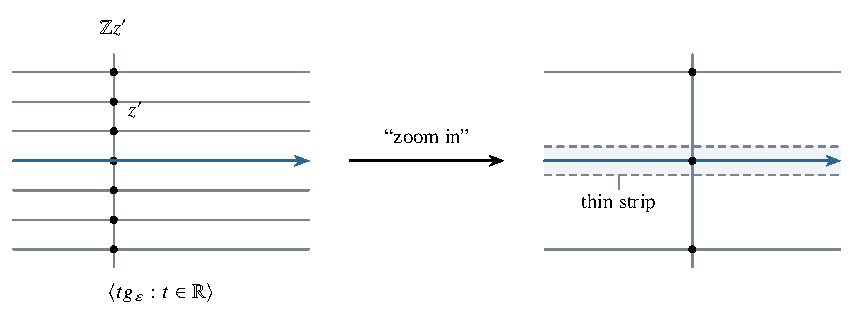
\includegraphics[width=0.88\linewidth]{note1-fig-02.pdf}

\end{figure}

If there are elements $z'\in G$ arbitrarily close to $\langle t g_\varepsilon:t\in\mathbb R\rangle$, then, since $G$ is closed, $G=\mathbb C$. Otherwise, choose a thin strip with no element of $G$ in the strip apart from $\langle t g_\varepsilon:t\in\mathbb R\rangle$. The interior and exterior of the strip form a separation. This is impossible, so $z_0\in G$, a contradiction. Hence $G=\mathbb C$.

\paragraph{Case 2.}
Suppose there is no $\varepsilon>0$ such that $B_\varepsilon(0)\cap G$ has no two linearly independent elements. Choose
\[
\varepsilon_1<\varepsilon_2<\varepsilon
\]
small enough, and let
\[
g_1\in\partial B_{\varepsilon_1}(0)\cap G,
\qquad
g_2\in\partial B_{\varepsilon_2}(0)\cap G,
\]
with $g_1,g_2$ linearly independent. Then the grid \(\mathbb Zg_1+\mathbb Zg_2\subset G,\)
and $z_0$ belongs to a box of diameter less than $\varepsilon$. Hence $z_0$ is a limit point, so $z_0\in G$ and $G=\mathbb C$.

\begin{figure}[htbp]
  \centering
  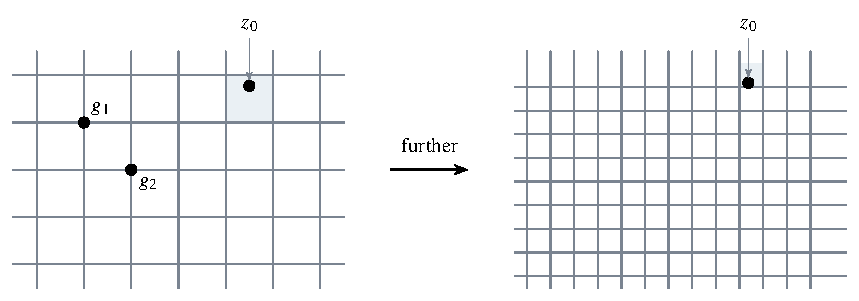
\includegraphics[width=0.82\linewidth]{note1-fig-03.pdf}

\end{figure}

Therefore the only connected closed additive subgroups of $(\mathbb C,+)$ are
\[
\mathbb C,\qquad\langle0\rangle,
\qquad\left\langle tz:t\in\mathbb R\right\rangle.
\]
Now, if \(G=\left\langle re^{i\theta}:re^{i\theta}\in G\right\rangle\)
is a connected closed subgroup of $\mathbb C^*$, then
\[
\exp^{-1}(G)=\{\log r+i(\theta+2\pi k):re^{i\theta}\in G,\ k\in\mathbb Z\}
\]
is a closed subgroup of $(\mathbb C,+)$. Its identity component is a connected closed additive subgroup, and its exponential image is $G$.

\textbf{Remark.}
Notice again that the geometry of $\mathbb C$ is the connection between the additive and multiplicative substructures of the field $\mathbb C$. We did not name the tools on their first invocation because we intend that they should become second nature.
% BLOG-CONTENT-END
\end{document}
